\documentclass[main]{subfiles}

\begin{document}


\chapter{Simulaciones del modelo f\'isico}
\label{chap:simulador}

Luego de desarrollado un modelo f\'isico resulta fundamental disponer de un entorno para realizar simulaciones. Las razones para construir un simulador son evidentes. En primer lugar resulta fundamental para comprobar que el modelo realizado se comporta acorde a lo que uno espera a priori del sistema. Para este tipo de pruebas se trabajar\'a con las situaciones m\'as sencillas en las cuales se puede calcular la trayectoria trivialmente. El segundo objetivo del simulador es poder conocer el comportamiento de nuestro sistema frente a algunas acciones de control determinadas. Por ejemplo conocer la trayectoria que desarrolla el cuadric\'optero si accionamos solamente uno de los motores o cualquier combinaci\'on que sea pertinente de estudio. Por \'ultimo, el simulador ser\'a clave para testear y mejorar los algoritmos de control desarrollados. Previo a testear con el sistema real y a fin de evitar da\~nos sobre el mismo, se deben verificar dichos algoritmos en el simulador. Por los motivos expresados es necesario que el simulador represente fielmente el modelo f\'isico y se comporte acorde a la realidad. \\

\section{Estructura del Simulador}


El simulador se compone de dos partes fundamentales. La primera es el lazo abierto, es decir las ecuaciones que gobiernan al cuadric\'optero, donde se consideran como entradas las velocidades angulares del sistema sobre las cuales realizaremos las acciones de control y como salidas tenemos el vector de estados del sistema en todos los instantes desde el tiempo inicial establecido en la simulaci\'on hasta el tiempo final. La otra parte se encarga de simular las acciones de control.

\subsection{Lazo Abierto}

La estructura que se eligi\'o para desarrollar esta secci\'on se corresponde en buena forma con el camino que se recorri\'o para determinar el modelo f\'isico. El lazo abierto consta de tres bloques principales. En primer lugar tenemos un bloque encargado de generar las fuerzas y momentos a partir de las velocidades angulares de las h\'elices. Luego tenemos un bloque que se encarga de resolver la din\'amica del sistema, y un cuarto bloque encargado de la cinem\'atica. En la figura \ref{fig:lazo_abierto} se observa la estructura global del lazo abierto. En la figura \ref{fig:vista} se observa una captura de pantalla que representa la vista general de la parte encargada de simular el lazo abierto.
\begin{figure}[h!]
	\centering
	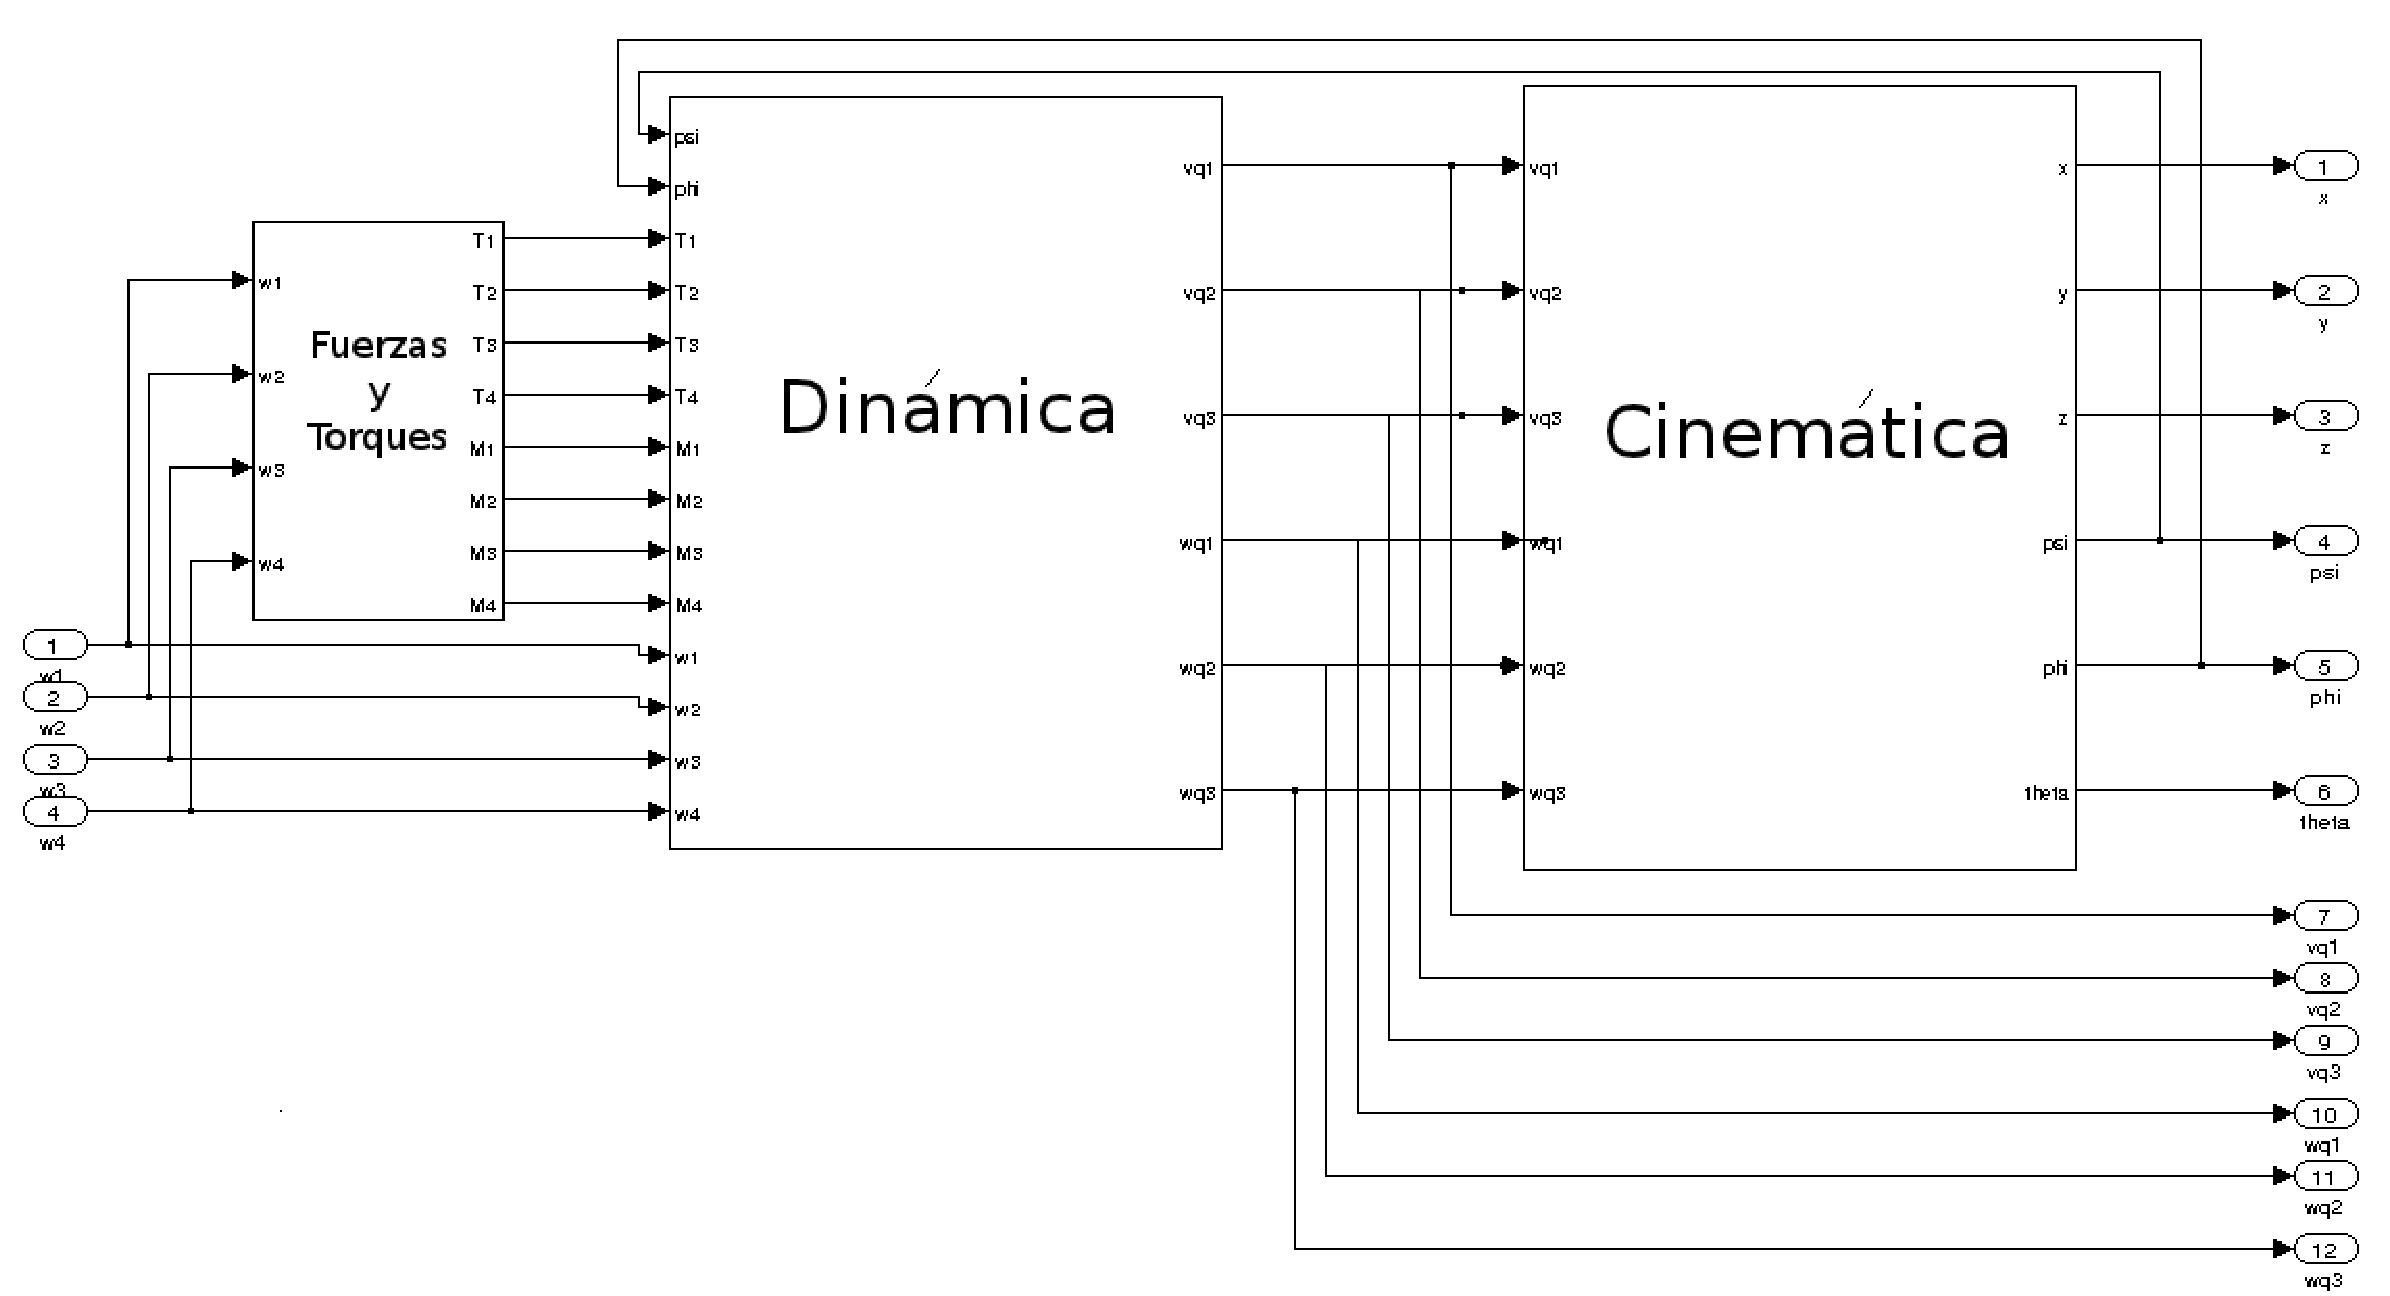
\includegraphics[width=1\textwidth]{./pics_simulador/lazo_abierto.pdf}
	\caption{Bloque de lazo abierto}
	\label{fig:lazo_abierto}
\end{figure}

\begin{figure}[h!]
	\centering
	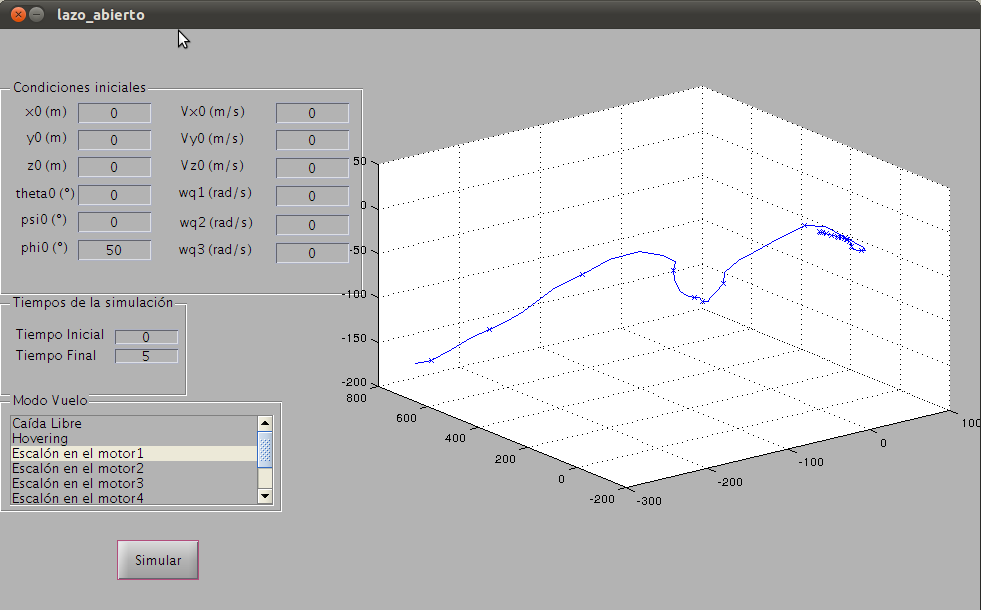
\includegraphics[width=1\textwidth]{./pics_simulador/vista.png}
	\caption{Interfaz del simulador de lazo abierto}
	\label{fig:vista}
\end{figure}
\subsubsection{Cinem\'atica}

En la figura \ref{fig:cinematica} se puede observar un diagrama de bloques de la parte del sistema que transforma las velocidades lineales y angulares en posiciones y \'angulos de Euler. Se distinguen dos sub-bloques principales, uno encargado de devolver la  posici\'on y otro encargado de devolver los \'angulos de Euler
\begin{figure} [h!]
  \centering
  \subfloat[Bloque cinem\'atica]{\label{fig:cinematica}
  		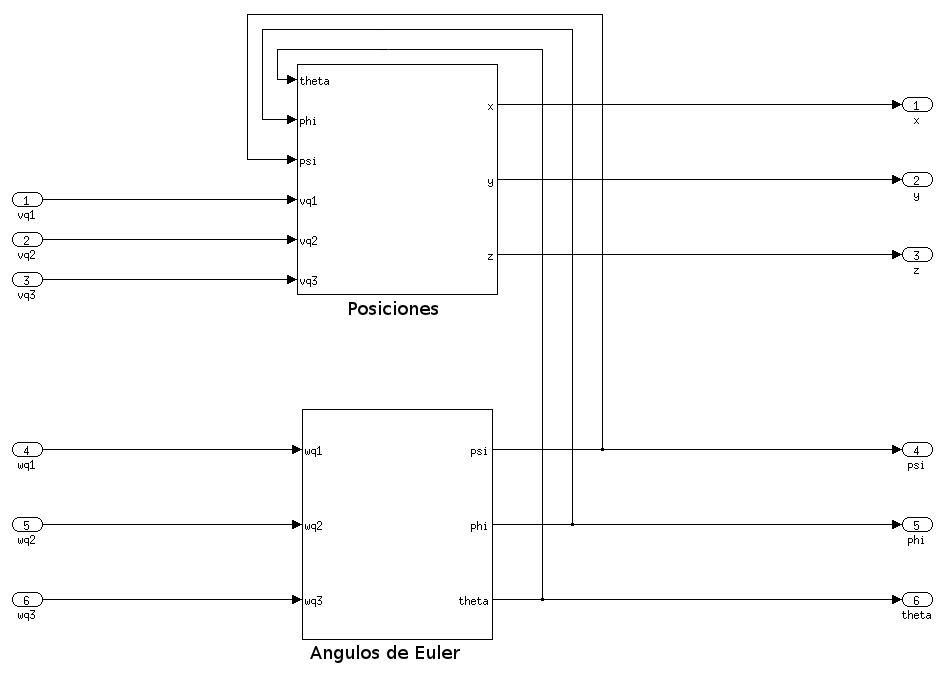
\includegraphics[width=0.6\textwidth]
  			{./pics_simulador/cinematica.png}}
  \subfloat[Bloque din\'amica]{\label{fig:dinamica}
  		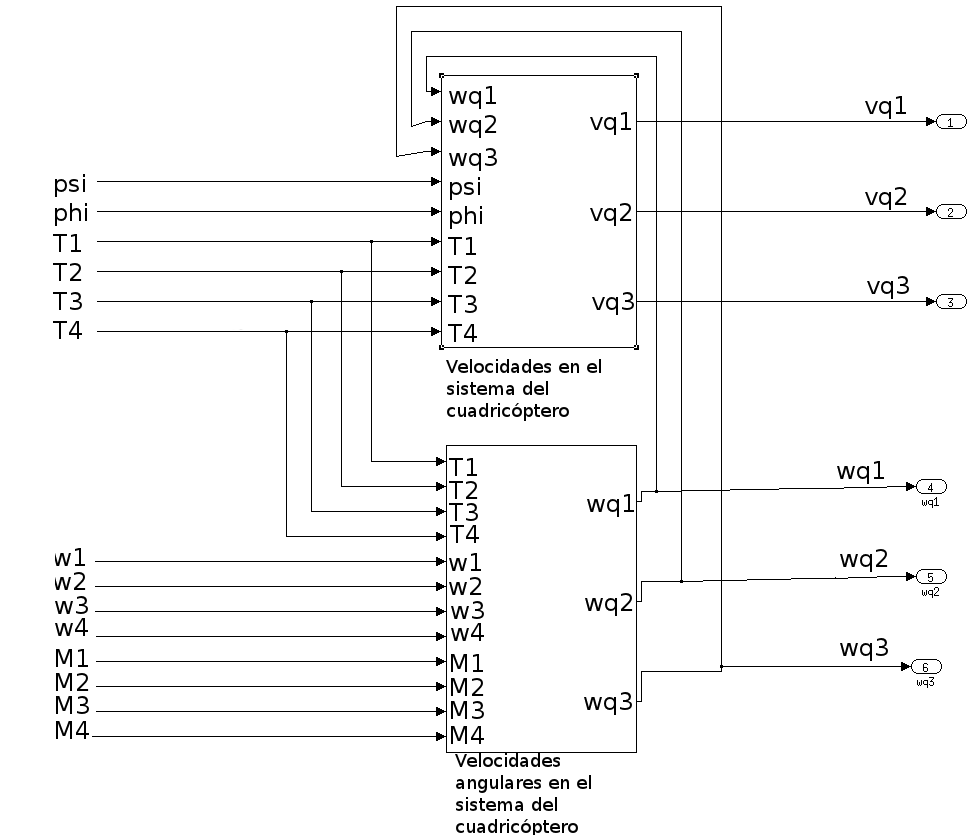
\includegraphics[width=0.5\textwidth]
  			{./pics_simulador/dinamica.png}}
  \caption{Bloques en mayor detalle}
  \label{fig:bloques}
\end{figure}



\subsubsection{Din\'amica}

Al igual que el bloque anterior, se divide este en dos sub-bloques m\'as (ver figura \ref{fig:dinamica}): El que devuelve las velocidades angulares, y el que devuelve las velocidades lineales. 

\subsection{Lazo cerrado}

Como se explica en el cap\'itulo \ref{chap:linealizacion}, para tratar las trayectorias circulares en el plano horizontal es necesario introducir un cambio de variables en el sistema. Este cambio de variables consiste en expresar la posici\'on del cuadric\'optero en el sistema $S_q$ solidiario a \'el y considerando como origen el centro de la trayectoria circular, en lugar de expresar la posici\'on en el sistema cartesiano inercial. Esta modificaci\'on implica realizar un cambio en el modelo para trabajar con dichas trayectorias, simplemente se agrega una matriz de rotaci\'on para trabajar con la posci\'on expresada en el sistema solidario al cuadric\'optero.\\ 

Desde la interfaz gr\'afica se puede seleccionar el tipo de trayectoria que se desea realizar y los valores de las variables de estado con las que se desea realizar dicha trayectoria\footnote{Evidentemente existen restricciones a la hora de elegir las variables de estado, a modo de ejemplo no seremos capaces de controlar una trayectoria en linea recta si las velocidades angulares no son nulas}. Las velocidades angulares objetivo para cada motor ser\'an determinadas a partir de la informaci\'on anterior. Al igual que en el simulador de lazo abierto, se tiene la posibilidad de establecer tanto el tiempo inicial de la simulaci\'on como las condiciones iniciales. La matriz de realimentaci\'on quedar\'a determinada por la trayectoria.\\

Fue necesario adem\'as acotar la velocidad angular de los motores ya que esta no puede tener cualquier valor, para esto se agregaron los bloques de saturaci\'on a la entrada del subsistema que representa la din\'amica del cuadric\'optero.\\

Como se explic\'o en la secci\'on \ref{chap:general} el control ser\'a realizado con un microprocesador, esto implica que las acciones de control no podr\'an ser modificadas en forma continua, cada cierto per\'iodo se indicar\'a un nuevo valor de velocidad angular para cada motor. Del mismo modo, no se tiene conocimiento del estado en todo instante sino que se tienen datos cada un cierto intervalo de tiempo (no necesariamente igual al per\'iodo con el cual se act\'ua sobre los motores). Estas consideraciones hacen necesaria una modificaci\'on en el sistema que hasta ahora hab\'ia sido considerado como continuo, es necesario convertir el sistema de tiempo continuo desarrollado a un sistema de tiempo discreto. Dicha modificaci\'on se logra sustituyendo los bloques integradores y derivadores que formaban parte del sistema por integradores y derivadores discretos con un per\'iodo de muestreo que tambi\'en puede ser impuesto desde la interfaz gr\'afica. En la figura \ref{fig:t_muestreo} se puede observar la misma trayectoria para tres tiempos de muestreo diferentes. En dicha trayectoria se muestra la subida del cuadric\'optero desde la altura inicial $z=0m$ hasta $z=3m$. 
 
\begin{figure} [h!]
  \centering
  \subfloat[Ts=50ms]{\label{fig:50ms}
  		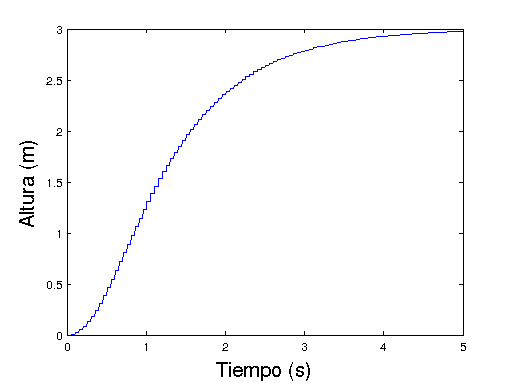
\includegraphics[width=0.35\textwidth]
  			{./pics_simulador/50ms.png}}
  \subfloat[Ts=500ms]{\label{fig:500ms} 
  		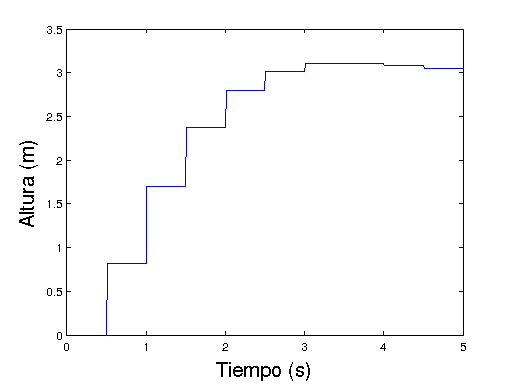
\includegraphics[width=0.35\textwidth]
  			{./pics_simulador/500ms.png}}
	  \subfloat[Ts=1s]{\label{fig:1000ms} 
  		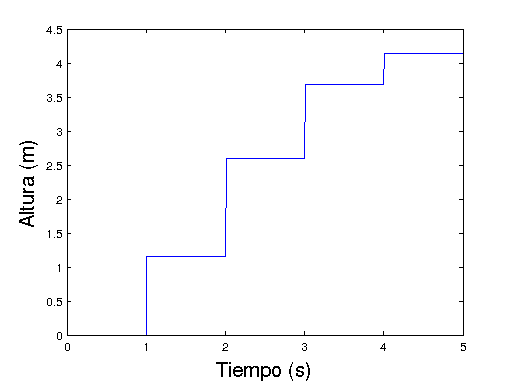
\includegraphics[width=0.35\textwidth]
  			{./pics_simulador/1000ms.png}} 
  \caption{Trayectoria de ascenso del cuadric\'optero desde $z=0$ a $z=3$}
  \label{fig:t_muestreo}
\end{figure} 
 
Se observa claramente un deterioro de la performance en la subida al aumentar el per\'iodo de muestreo y de acci\'on sobre los motores. Por dicho motivo es importante incluir esta variable a la hora de realizar diversas simulaciones ya que el sistema real debe realizar una gran cantidad de operaciones y si bien su capacidad es considerable no es infinita. Esto puede producir que se tenga acotado inferiormente el per\'iodo de muestreo.\\

Por \'ultimo, se desea incluir la posibilidad de agregar ruido a los estados medidos y perturbaciones en las velocidades angulares de los motores. Las medidas que se obtienen de los sensores no son exactas, por dicho motivo la posibilidad de agregar ruido es muy interesante de modo de testear la robustez del controlador implementado. Asimismo, la velocidad angular de los motores no es exactamente la que se espera de acuerdo a la caracterizaci\'on de los motores realizada (ver cap\'itulo \ref{chap:test_motores}), por el contrario, se producen variaciones en la velocidad angular de los mismos dada una velocidad angular objetivo.
  \begin{figure}[h!]
	\centering
	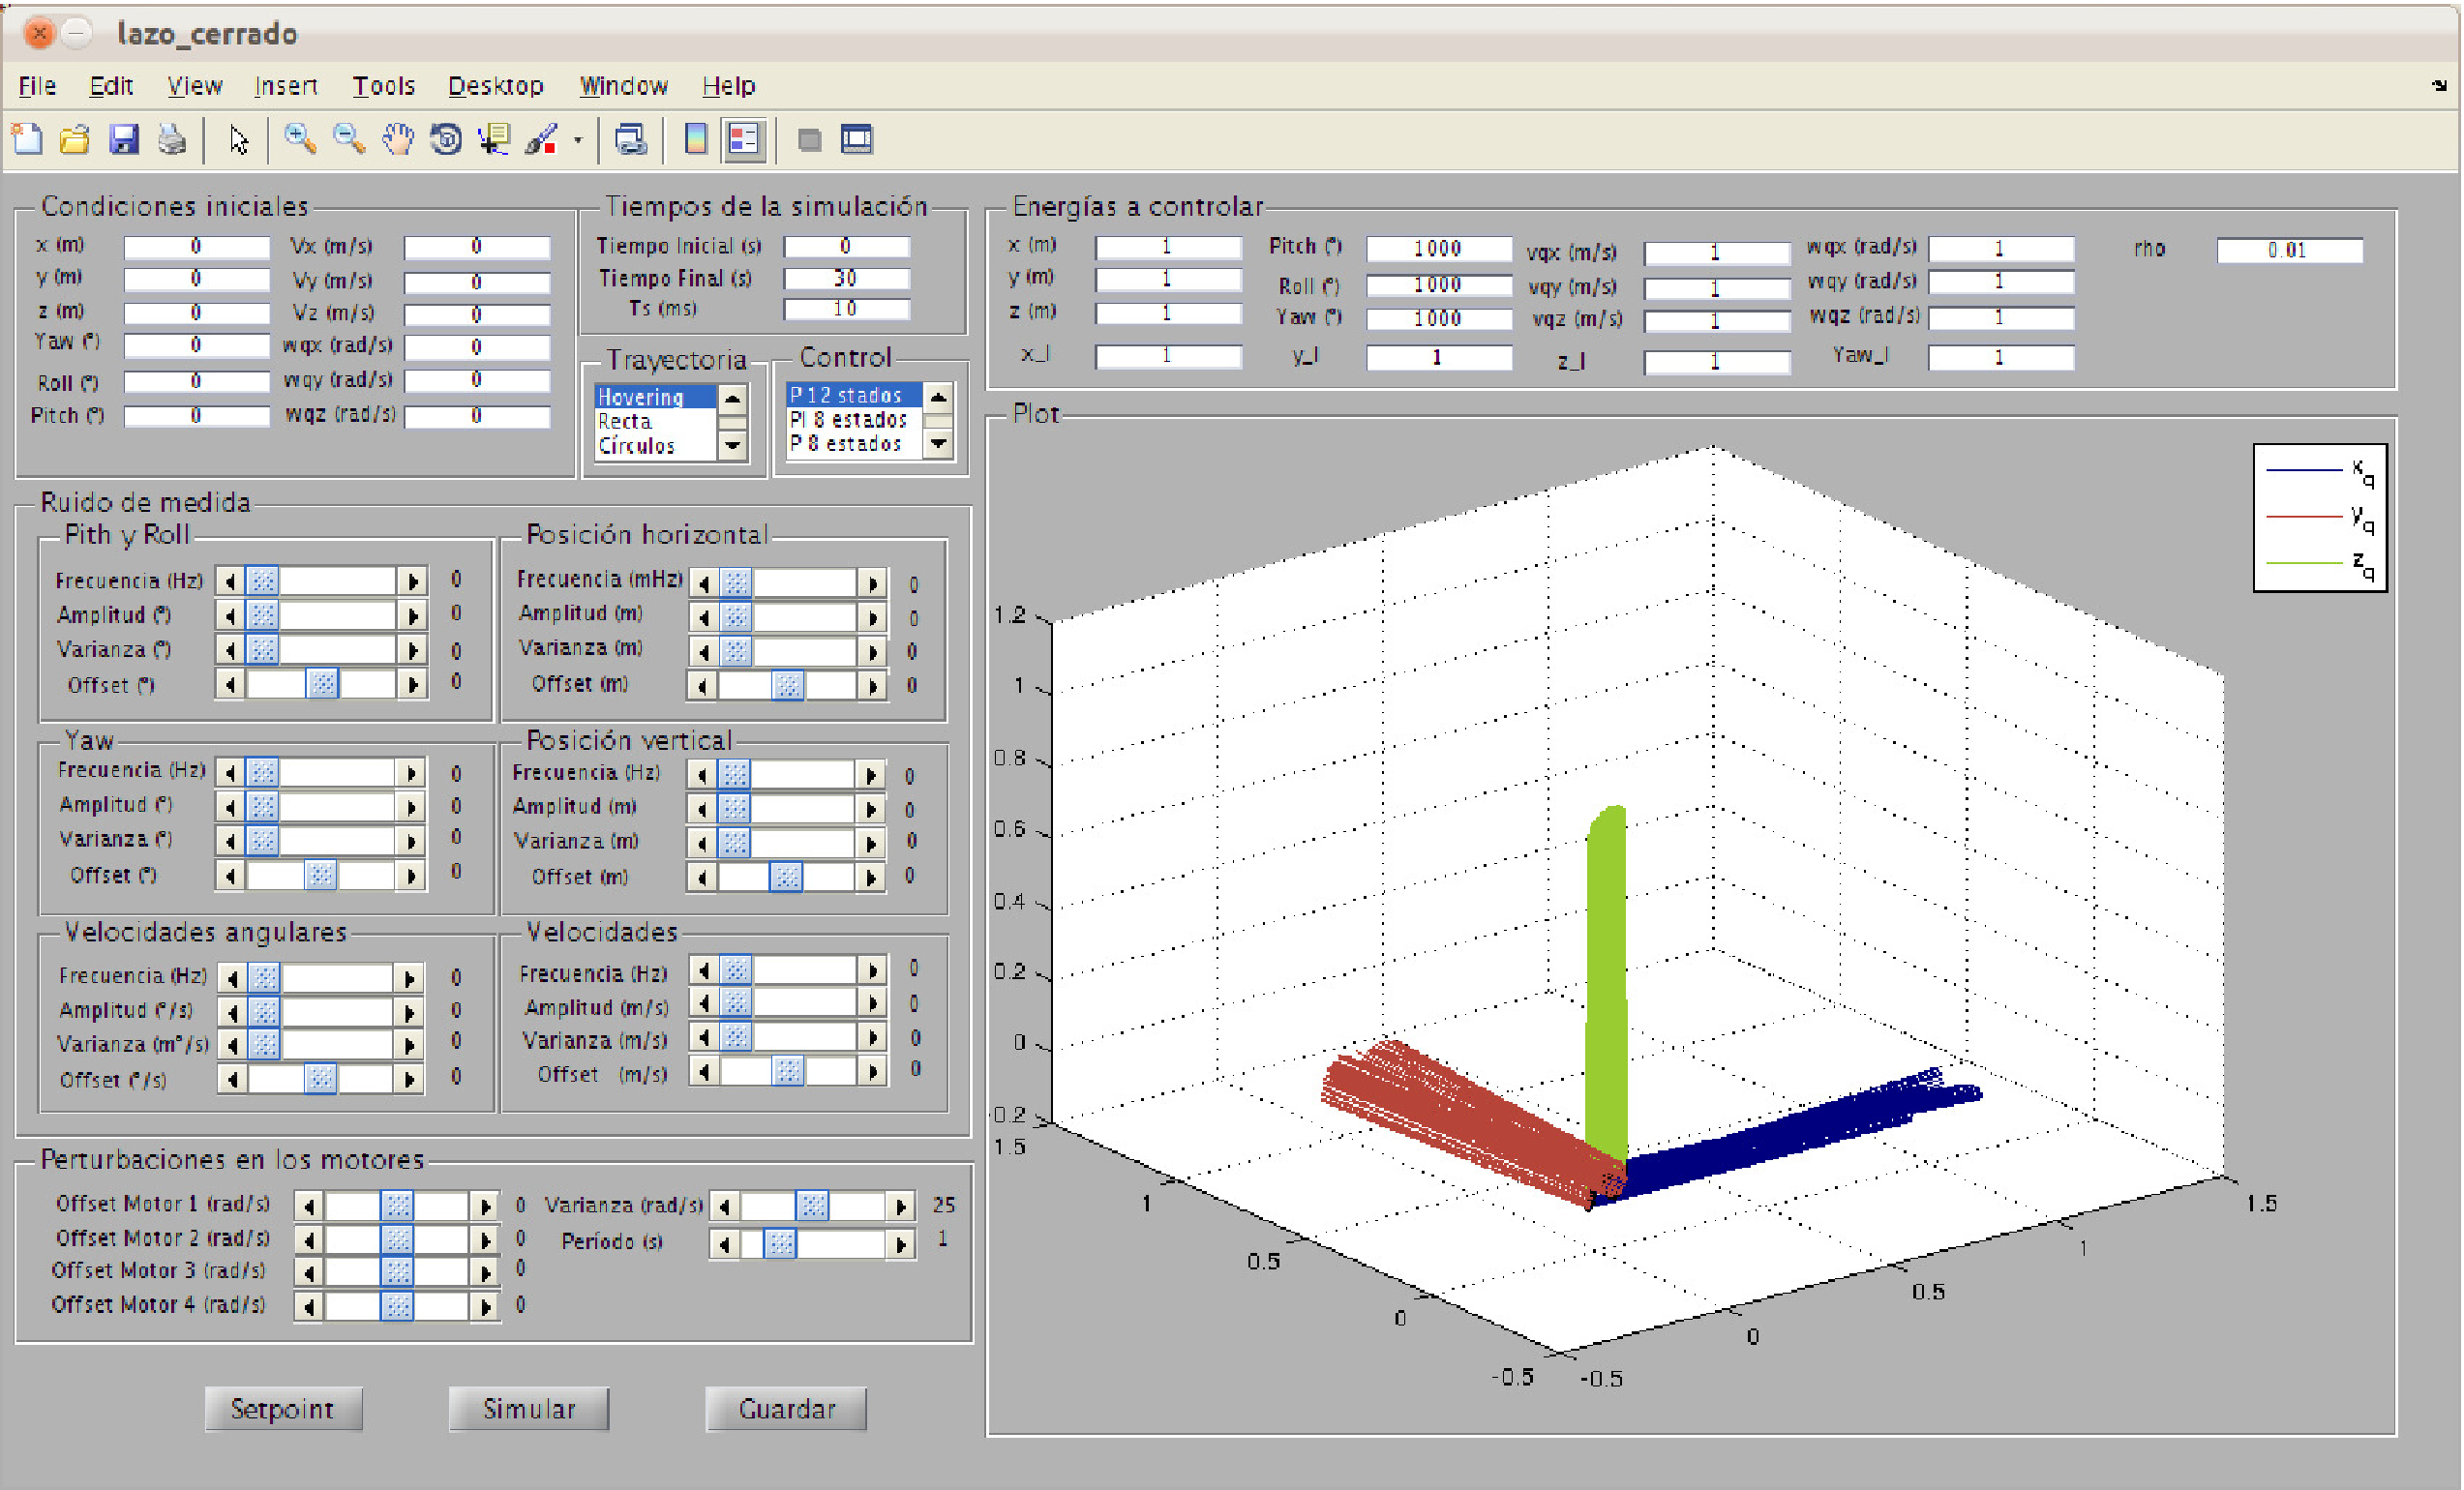
\includegraphics[width=1\textwidth]{./pics_simulador/vistac.pdf}
	\caption{Interfaz del simulador de lazo cerrado}
	\label{fig:vistac}
\end{figure}

\section{Simulaciones}
En esta secci\'on procedermos a realizar algunas simulaciones a fin de verificar que los resultados arrojados se corresponden con lo esperado a priori. 

\subsubsection{Ca\'ida libre con velocidad inicial nula}

Se simula una ca\'ida libre con condiciones iniciales nulas excepto la altura que se fija a $100m$. El tiempo de simulaci\'on considerado es de tres segundos. En la figura \ref{fig:clv0} se observa la trayectoria obtenida. En este caso se grafica uno de cada veinte puntos obtenidos. La misma se corresponde con lo que se espera a priori: puntos equiespaciados en el tiempo se encuentran cada vez m\'as apartados a medida que transcurre el tiempo. En la figura \ref{fig:zcl} se representa la altura en funci\'on del tiempo. La altura final es $z_f=55.855m$. La altura en una ca\'ida libre puede calcularse como $z(t)=-\frac{gt^2}{2}+Z_0$. En este caso se obtiene $z(3)=55.855m$.



\begin{figure} [h!]
  \centering
  \subfloat[Trayectoria de caida libre con velocidad inicial nula]{\label{fig:clv0}
  		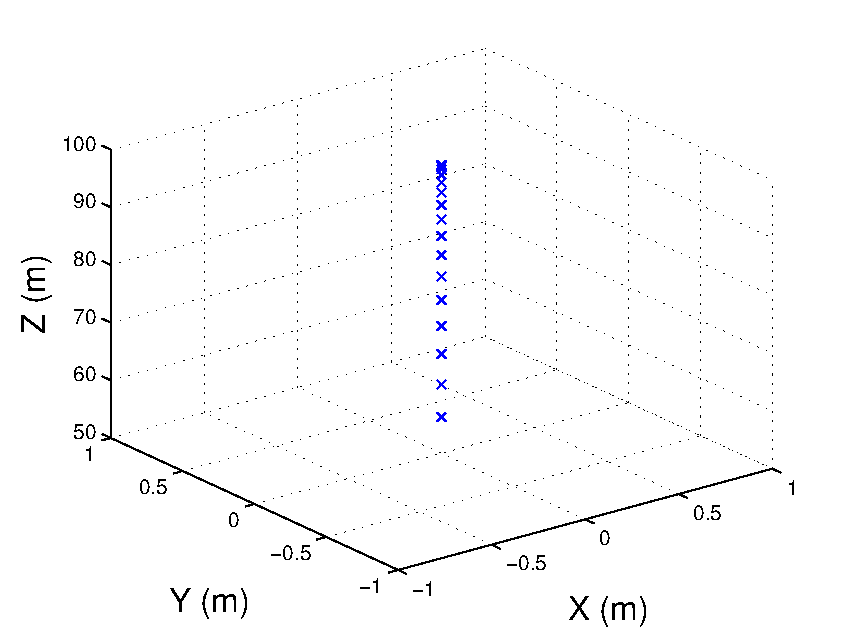
\includegraphics[width=0.5\textwidth]
  			{./pics_simulador/clv0.pdf}}
  \subfloat[Altura en funci\'on del tiempo]{\label{fig:zcl} 
  		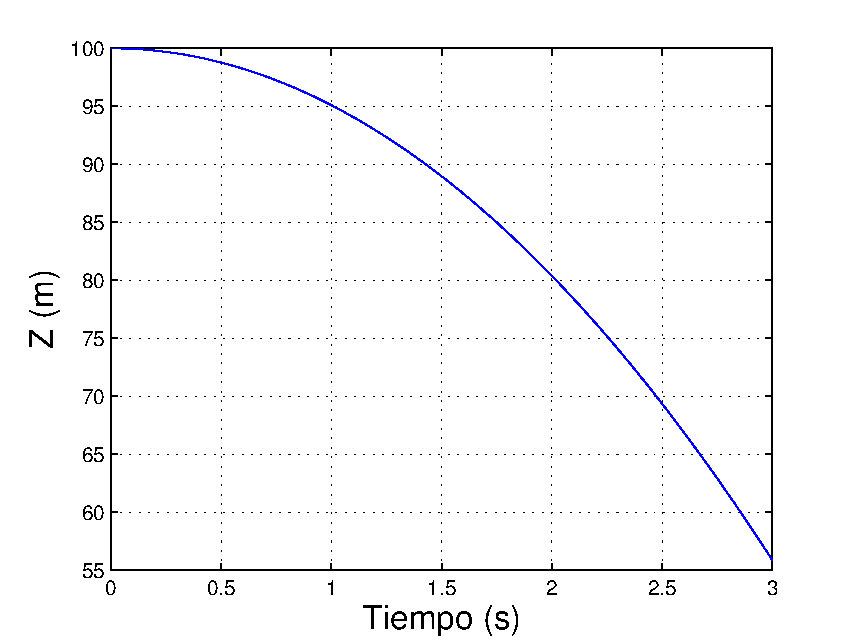
\includegraphics[width=0.5\textwidth]
  			{./pics_simulador/clz.pdf}}
 
  \caption{Caida libre con velocidad inicial nula}
  \label{fig:caida_libre}
\end{figure}

\subsubsection{Ca\'ida libre con velocidad inicial}
Se realiza la misma simulaci\'on que en la secci\'on anterior excepto que se inicia el vuelo con $V_0 = 1ms^{-1}\vec{i}+3ms^{-1}\vec{k}$. Los resultados de la simulaci\'on pueden encontrarse expresados graficamente en la figura \ref{fig:caida_libre_vi}. La coordenada de la posici\'on seg\'un $\vec{i}$ aumenta con el tiempo con pendiente igual a la velocidad inicial. La altura cumple que $z(t)=-\frac{gt^2}{2}+3ms^{-1}t+Z_0$. Por lo tanto la misma aumenta hasta un tiempo  $t_{max} / \dot{z}(t)=0$. Lo cual implica que $t_{max}=\frac{3ms^{-1}}{g}\approx0.31s$. Por otra parte tiempo para el cual se da el m\'aximo en la simulaci\'on es $t_{max_{sim}} = 0.306s$. Considerando que las simulaciones se realizan con un paso variable el cual puede ser de hasta $0.01s$ se considera un resultado aceptable. El siguiente valor para el tiempo simulado es $0.316s$, por lo tanto es razonable que dicho valor se presente en $t_{max_{sim}}$. La altura m\'axima te\'orica vale $z_{max_{teo}}=100.459m$, la altura m\'axima obtenida a trav\'es de la simulaci\'on es igual\footnote{Considerando tres cifras despu\'es de la coma}. A partir de este punto tenemos una ca\'ida libre como la que ya estudiamos en el caso anterior. Las alturas finales, tanto en la simulaci\'on como en la teor\'ia valen $64.885m$.

\begin{figure} 
  \centering
  \subfloat[Trayectoria de caida libre con velocidad $V_0 = 1ms^{-1}\vec{i}+3ms^{-1}\vec{k}$]{\label{fig:clv1}
  		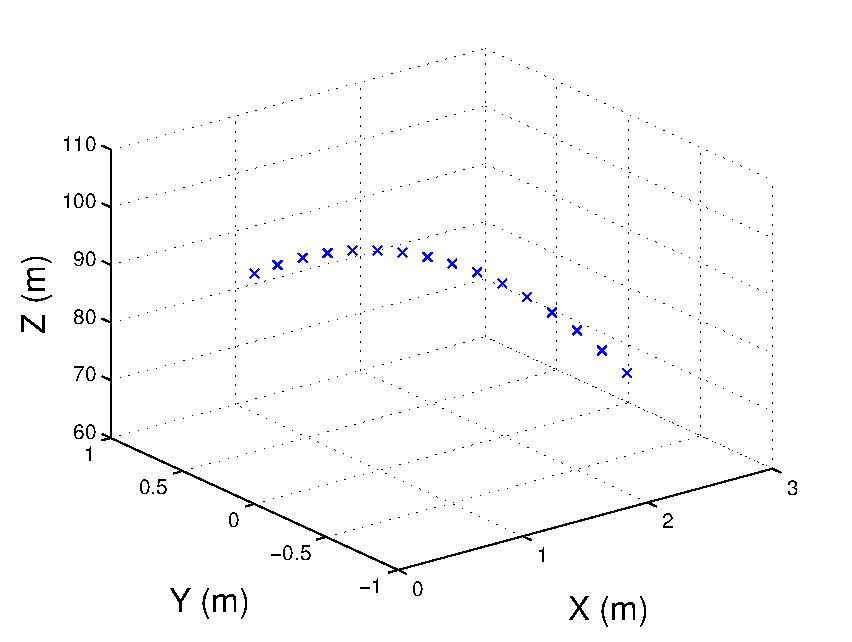
\includegraphics[width=0.35\textwidth]
  			{./pics_simulador/clv1.pdf}}
  \subfloat[Altura en funci\'on del tiempo]{\label{fig:clzv1} 
  		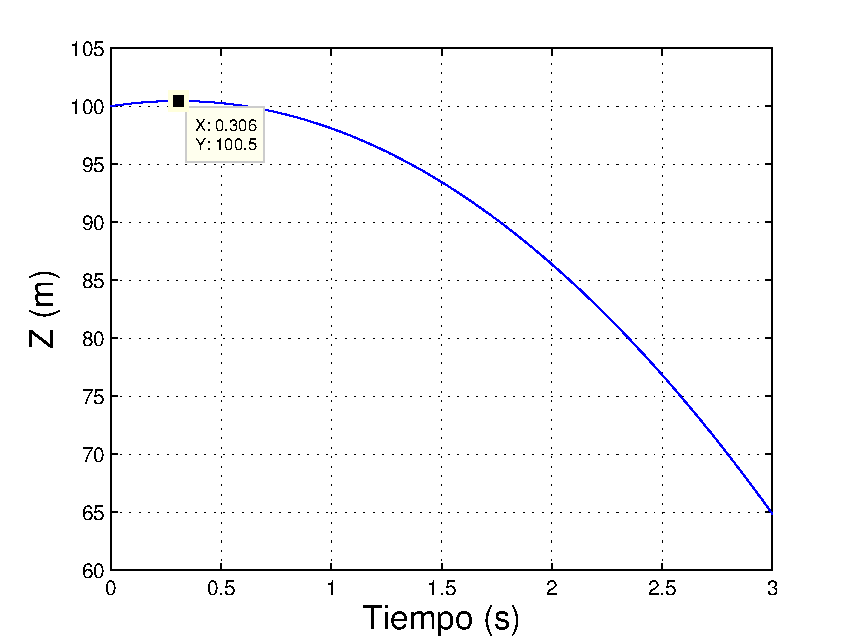
\includegraphics[width=0.35\textwidth]
  			{./pics_simulador/clzv1.pdf}}
   \subfloat[Desplazamiento hacia el Norte en funci\'on del tiempo]{\label{fig:clxv1} 
  		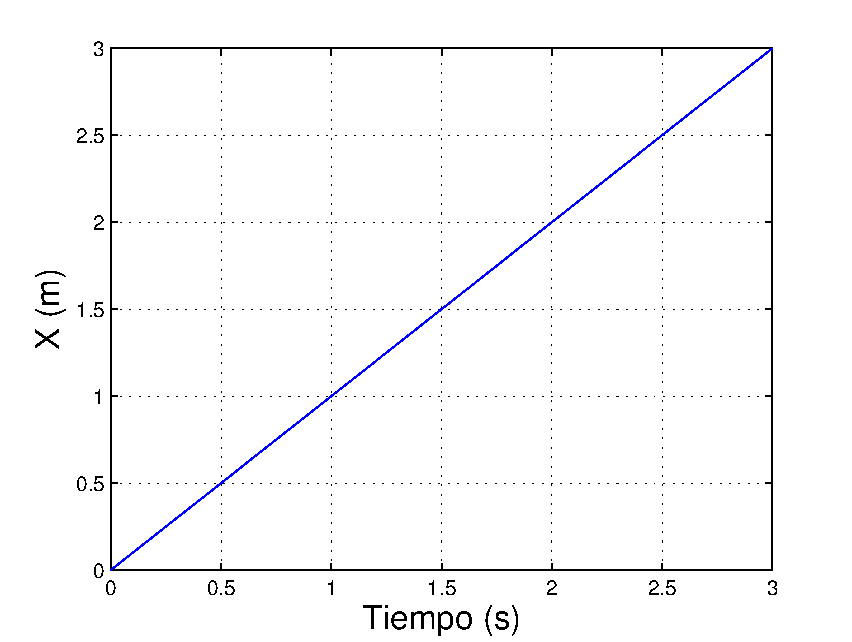
\includegraphics[width=0.35\textwidth]
  			{./pics_simulador/clx1.pdf}}   			
 
  \caption{Caida libre con velocidad inicial no nula}
  \label{fig:caida_libre_vi}
\end{figure}


\subsubsection{Condici\'on de Hovering}

Se aplica una fuerza constante en los cuatro motores tal que la resultante es igual al peso. Las condiciones iniciales son todas nulas, excepto $Z_0=10m$. Se logra el equilibrio mec\'anico. Todas las variables permanecen constantes. Se simula durante diez segundos

\subsubsection{Escal\'on en los cuatro motores}
Con condiciones iniciales nulas, en condici\'on de hovering se aumenta la velocidad angular de los motores en $100 rads^{-1}$ en $t=5s$. Se simula durante diez segundos. En la figura \ref{fig:escalon} se presentan gr\'aficamente los resultados obtenidos en la simulaci\'on. La altura m\'axima alcanzada por el cuadric\'optero en la simulaci\'on es de $93.61m$ mientras que en la teor\'ia dicha altura es de $93.78m$. Nuevamente la diferencia entre el valor simulado y el esperado difieren de manera despreciable y es atribuible a aproximaciones realizadas.

\begin{figure} [h!]
  \centering
  \subfloat[Altura en funci\'on del tiempo]{\label{fig:subidaz}
  		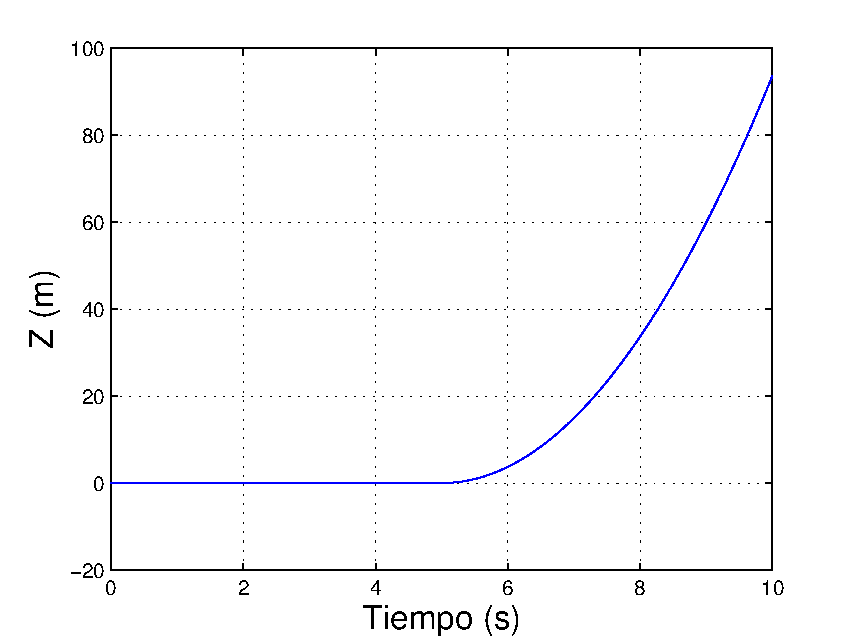
\includegraphics[width=0.5\textwidth]
  			{./pics_simulador/subidaz.pdf}}
   \subfloat[Trayectoria]{\label{fig:subida} 
  	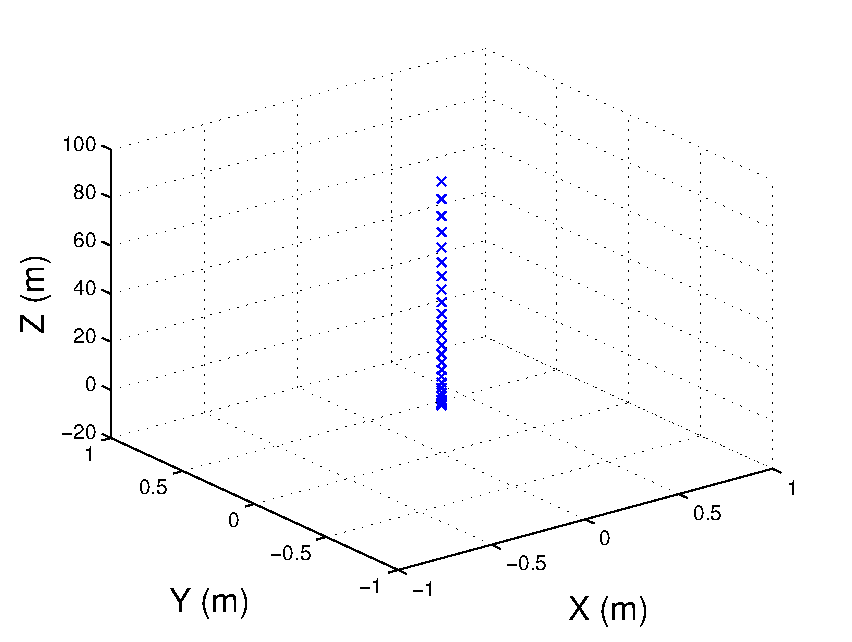
\includegraphics[width=0.5\textwidth]
  			{./pics_simulador/subida.pdf}} 
  \caption{Escal\'on en los cuatro motores}
  \label{fig:escalon}
\end{figure}

\subsubsection*{Cambio en el Pitch y el Roll}
Con condiciones iniciales nulas excepto la altura fijada en $z=10$, se realiza un giro seg\'un $\vec{i}_q$ y seg\'un $\vec{j}_q$. En el primer caso se aumenta la velocidad del motor 2 en tres radianes por segundo y se disminuye la velocidad del motor 4 en la misma cantidad. Para la segunda simulaci\'on se aumenta en tres radianes por segundo la velocidad del motor 3 y se disminuye en la misma cantidad la velocidad del motor 1. Los resultados obtenidos se muestran en la figura \ref{fig:giros}

\begin{figure} 
  \centering
  \subfloat[Roll funci\'on del tiempo]{\label{fig:roll}
  		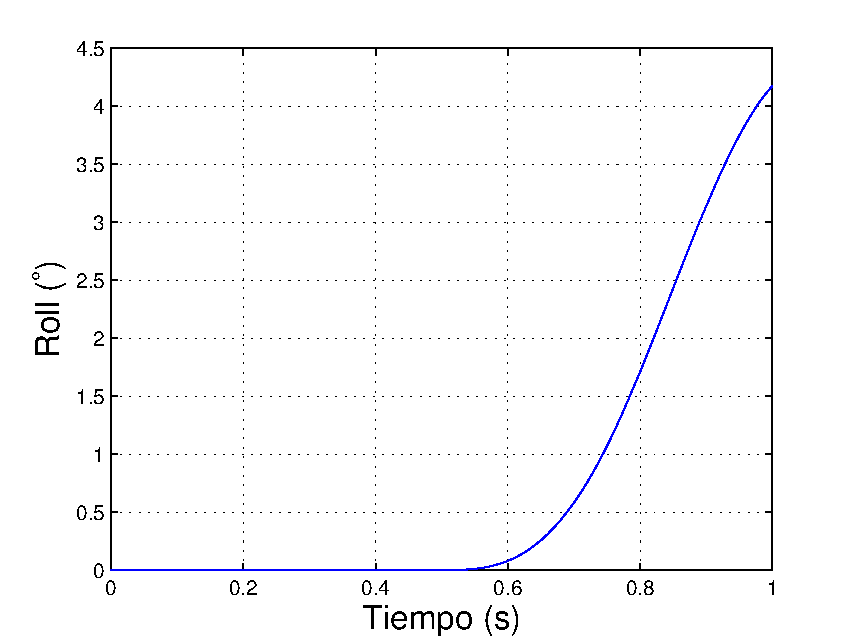
\includegraphics[width=0.5\textwidth]
  			{./pics_simulador/roll.pdf}}
   \subfloat[Pitch funci\'on del tiempo]{\label{fig:pitch} 
  	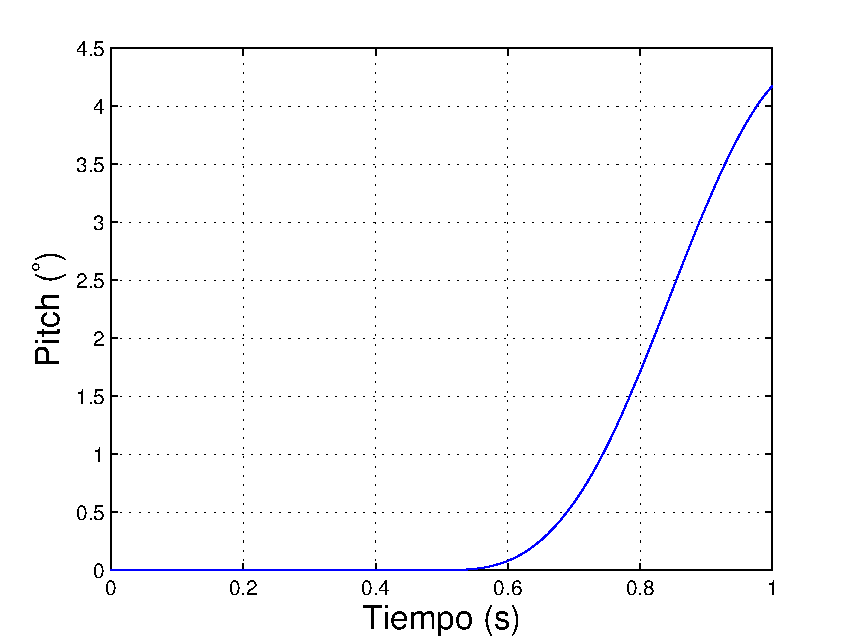
\includegraphics[width=0.5\textwidth]
  			{./pics_simulador/pitch.pdf}} 
  \caption{Aumento en los \'angulos de Pitch y Roll}
  \label{fig:giros}
\end{figure}

En estos dos casos tambi\'en se obtiene un resultado acorde a lo esperado. En ambos casos el \'angulo aumenta de forma cuadr\'atica en la zona donde el \'angulo es inferior a los dos grados, en esta zona puede despreciarse el momento realizado por el peso, por lo tanto se tiene una aceleraci\'on angular constante, lo cual explica el comportamiento del \'angulo. Para \'angulos superiores dicho torque del peso comienza a ser considerable respecto del torque producido por los motores y se observa que el \'angulo crece con menor pendiente.

\subsubsection{Giro seg\'un el eje $\vec{k}$}

En las mismas condiciones que la simulaci\'on anterior, en el tiempo $t=5s$ se aumenta repentinamente la velocidad angular de los motores que rotan en sentido horario con un valor tal que la fuerza de cada uno de esos motores aumenta en $1N$. Para los motores que rotan en sentido anti-horario se disminuye la velocidad angular de forma que la fuerza de cada uno de ellos disminuye $1N$. Estas velocidades son $349.88rads^{-1}$ y $278.09rads^{-1}$ respectivamente. La fuerza neta permanece constante y el momento seg\'un los versores $\vec{i_q}$ y $\vec{j_q} $ es nulo. Sin embargo aparece un torque positivo seg\'un el versor $\vec{k_q}$.\\

En la figura \ref{fig:hovz} se presenta la altura en funci\'on del tiempo. La misma deber\'ia permanecer constante, sin embargo se observa una peque\~na diferencia en la altura de $2.3cm$. Esta diferencia es atribuida a la aproximaci\'on realizada al calcular las velocidades con las cuales deben girar los motores. Por otra parte en la figura \ref{fig:hovtheta} se observa como el \'angulo aumenta hasta el valor de $84.43 rad$. El torque neto vale $Q = 0.29Nm $. Por lo tanto en 5 segundos se debe rotar un \'angulo de $\theta_f=84.16rad$. Nuevamente se percibe una peque\~na diferencia entre el valor te\'orico y el simulado, pero dicho error es aceptable. 

\begin{figure} [h!]
  \centering
  \subfloat[Altura en funci\'on del tiempo]{\label{fig:hovz}
  		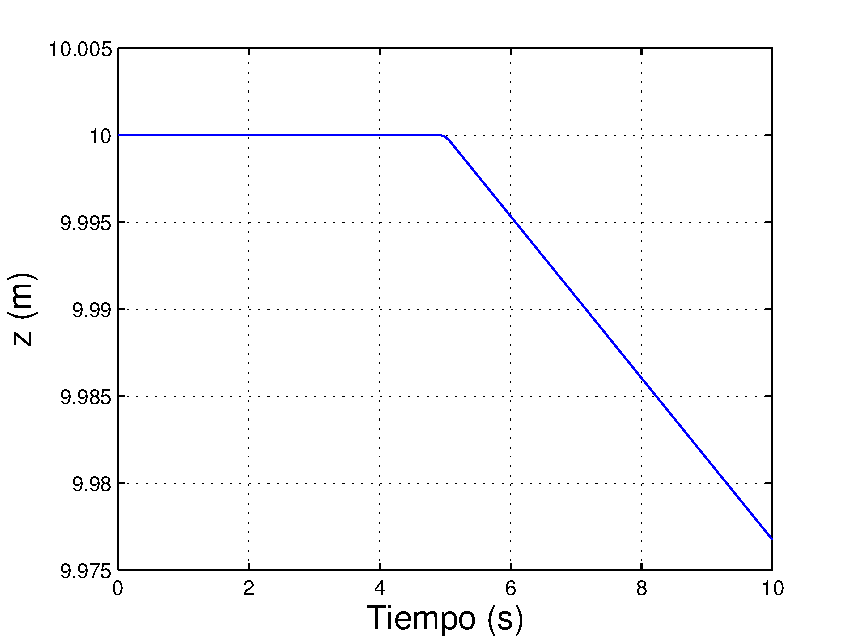
\includegraphics[width=0.5\textwidth]
  			{./pics_simulador/hovz.pdf}}
   \subfloat[\'Angulo de Yaw]{\label{fig:hovtheta} 
  	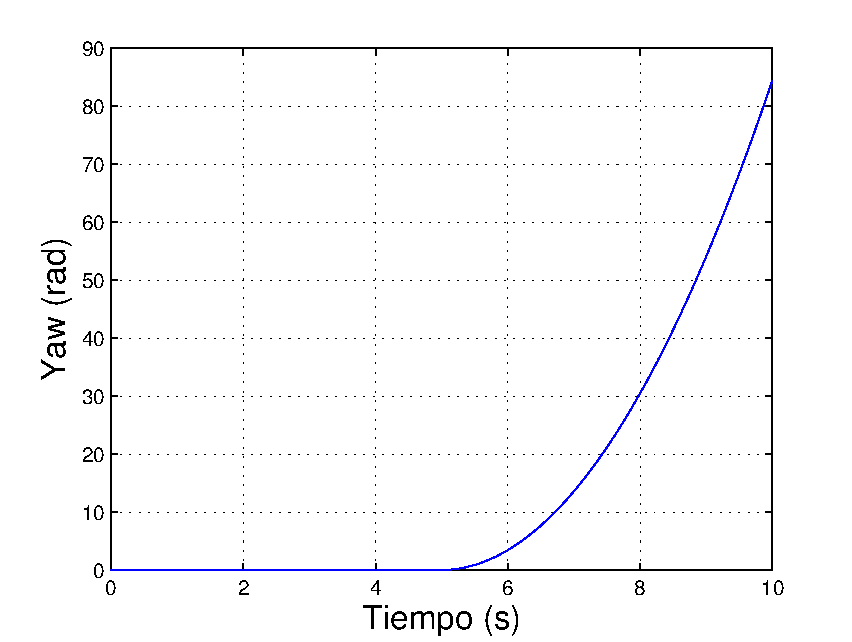
\includegraphics[width=0.5\textwidth]
  			{./pics_simulador/hov_theta.pdf}} 
  \caption{Giro seg\'un el $\vec{k_q}$}
  \label{fig:hov}
\end{figure}

Hasta aqu\'i hemos testeado el simulador en situaciones conocidas. Nos concentramos en analizar la caida libre y las cuatro acciones de control b\'asicas que se pueden realizar descriptas en \ref{chap:general}. De acuerdo a las pruebas realizadas puede afirmarse que su funcionamiento es el adecuado ya que en ninguna prueba se obtuvieron errores considerables. Sin embargo, es fundamental aclarar que hasta aqu\'i no es posible afirmar que el modelado del sistema sea adecuado, lo \'unico que puede concluirse es que el simulador representa fielmente las ecuaciones que han sido deducidas hasta el momento. Un error en las ecuaciones no se reflejar\'a hasta el momento de testear el cuadric\'optero. El trabajo realizado a la hora del modelado y la comparaci\'on con diversas bibliograf\'ias nos permite a esta altura estar convencidos de que dichas ecuaciones son adecuadas para modelar el sistema.

\end{document}